% Language: english, slovak
% Document type: article (bachelor thesis), report (master thesis)
%%
%% CHECK THE PLACE WITH "!!!!"
%%

%%
%% !!!! select one for BACHELOR THESIS
%%
%\documentclass[a4paper,english,12pt,appendix]{article}
\documentclass[a4paper,slovak,12pt,appendix]{article}

%%
%% !!!! select one for MASTER THESIS
%%
%\documentclass[a4paper,english,12pt,appendix]{report}
%\documentclass[a4paper,slovak,12pt,appendix]{report}
%\usepackage[bindingoffset=1.8cm,centering,includeheadfoot,margin=2.8cm]{geometry}

\usepackage{geometry}
 \geometry{
 a4paper,
 inner=30mm,
 outer=30mm,
 top=40mm,
 bottom=40mm,
 }

\usepackage{ifthen}
\newboolean{english}
\newboolean{bachelor}
%%
%% !!!! for MASTER THESIS set to FALSE
%%
\setboolean{bachelor}{true}

%%
%% !!!! for SLOVAK VERSION set to FALSE
%%
\setboolean{english}{false}



%%
%% Formats and Defs
%%
% Packages

\usepackage{array}
\usepackage{epsf}
\usepackage{epsfig}
\usepackage[utf8]{inputenc}
%\usepackage[utf8x]{inputenc}
\usepackage[T1]{fontenc}
\usepackage[slovak]{babel}
%\usepackage[IL2]{fontenc}
\usepackage{latexsym}
\usepackage{float}
\usepackage[usenames]{color}
\usepackage{newcent}
\usepackage{graphicx}
\usepackage{setspace}
%\onehalfspacing
\doublespace
\usepackage[numbers]{natbib}
\usepackage{url}
\usepackage{eso-pic}
\usepackage{listingsutf8}
\usepackage{verbatim}
\usepackage{moreverb}
\usepackage{microtype}
\usepackage[noauto]{chappg}
\usepackage{lmodern}
\usepackage[toc,title]{appendix}
\usepackage{libertine}
\usepackage{mathtools}
\usepackage{subfigure}
\usepackage{textcomp}
\usepackage{ucs}
\usepackage{dirtree}
\usepackage{enumerate}
%\usepackage[colorlinks=true,urlcolor=red,hyperfootnotes=false]{hyperref}
\usepackage{amsfonts}
\usepackage{enumitem}
\usepackage{multicol}
\usepackage{fancyhdr}
\usepackage{tikz}
% Language
\ifthenelse {\boolean{english}}
{
	\usepackage[english]{babel}

	\renewcommand{\lstlistingname}{Example}
	\renewcommand{\lstlistlistingname}{List of Examples}
}
{
	%\usepackage[slovak]{babel}
	%\usepackage[IL2]{fontenc}

	\renewcommand{\lstlistingname}{Ukážka}
	\renewcommand{\lstlistlistingname}{Zoznam ukážok}

}

% Section rules
\usepackage{sectsty}
\usepackage{times}
\usepackage{afterpage}

\newcommand\blankpage{%
    \null
    \thispagestyle{empty}%
   %addtocounter{page}{-1}%
    \newpage}
% Bookmarks

% black references
\usepackage[pdfborder={0 0 0}]{hyperref}

% red references
%\usepackage[colorlinks=true,linkcolor = black,urlcolor = black,citecolor=black]{hyperref}

% Colors
\definecolor{light-gray}{gray}{0.95}
\definecolor{gray}{gray}{0.2}
\definecolor{blue}{rgb}{0,0,1}
\definecolor{red}{RGB}{208,0,0}
\definecolor{green}{RGB}{0,134,38}
\definecolor{yellow}{rgb}{1,0.35,0}
\definecolor{black}{rgb}{0,0,0}
\definecolor{back}{RGB}{245,245,245}

% Listings settings
\lstdefinelanguage{lua}{
	morekeywords={and,break,do,else,elseif,end,false,for,function,if,in,local,nil,not,or,repeat,return,then,true,until,while},
	morekeywords={[2]arg,assert,collectgarbage,dofile,error,_G,getfenv,getmetatable,ipairs,load,loadfile,loadstring,next,pairs,pcall,print,rawequal,rawget,rawset,select,setfenv,setmetatable,tonumber,tostring,type,unpack,_VERSION,xpcall},
	morekeywords={[2]coroutine.create,coroutine.resume,coroutine.running,coroutine.status,coroutine.wrap,coroutine.yield},
	morekeywords={[2]module,require,package.cpath,package.load,package.loaded,package.loaders,package.loadlib,package.path,package.preload,package.seeall},
	morekeywords={[2]string.byte,string.char,string.dump,string.find,string.format,string.gmatch,string.gsub,string.len,string.lower,string.match,string.rep,string.reverse,string.sub,string.upper},
	morekeywords={[2]table.concat,table.insert,table.maxn,table.remove,	table.sort},
	morekeywords={[2]math.abs,math.acos,math.asin,math.atan,math.atan2,math.ceil,math.cos,math.cosh,math.deg,math.exp,math.floor,math.fmod,math.frexp,math.huge,math.ldexp,math.log,math.log10,math.max,math.min,math.modf,math.pi,math.pow,math.rad,math.random,math.randomseed,math.sin,math.sinh,math.sqrt,math.tan,math.tanh},
	morekeywords={[2]io.close,io.flush,io.input,io.lines,io.open,io.output,io.popen,io.read,io.tmpfile,io.type,io.write,file:close,file:flush,file:lines,file:read,file:seek,file:setvbuf,file:write},
	morekeywords={[2]os.clock,os.date,os.difftime,os.execute,os.exit,os.getenv,os.remove,os.rename,os.setlocale,os.time,os.tmpname},
	keywordstyle=\color{black},
	ndkeywordstyle=\color{black},
	commentstyle=\color{black},
	stringstyle=\color{gray},
	identifierstyle=\color{black},
	sensitive=true,
	morecomment=[l]{--},
	morecomment=[s]{--[[}{]]--},
	morestring=[b]",
	morestring=[d]',
    showstringspaces=false,
	backgroundcolor=\color{white},
	frame=single,
	frameround=ffff,
	captionpos=b,
	basicstyle=\scriptsize
}

\lstdefinelanguage{nil}{
  identifierstyle=\color{black}\ttfamily,
  sensitive=true,
  columns=flexible,
  backgroundcolor=\color{white},
  frame=single,
  frameround=ffff,
  captionpos=b,
  basicstyle=\scriptsize
}

\lstdefinelanguage{javascript}{
  keywords={typeof, new, true, false, catch, function, return, null, catch, switch, var, if, in, while, do, else, case, break},
  ndkeywords={class, export, boolean, throw, implements, import, this},
  sensitive=false,
  comment=[l]{//},
  morecomment=[s]{/*}{*/},
  morestring=[b]',
  morestring=[b]",
  keywordstyle=\color{blue}\normalfont,
	ndkeywordstyle=\color{black}\normalfont,
	commentstyle=\color{red}\ttfamily,
	stringstyle=\color{green}\ttfamily,
	identifierstyle=\color{gray},
	backgroundcolor=\color{white},
	frame=single,
	frameround=ffff,
	captionpos=b,
	basicstyle=\scriptsize
}

\lstdefinestyle{color}
	{identifierstyle=\color{green}\bfseries, commentstyle=\color{yellow}\bfseries, stringstyle=\color{blue}, keywordstyle=\color{red}\bfseries,morecomment=[l]{\#}}

\lstset{postbreak=\small>>\space,prebreak=\small>>,breakindent=13pt,breaklines=true,inputencoding=utf8,tabsize=2,showtabs=false,tab=$\to$,style=color,basicstyle=\footnotesize\ttfamily\normalfonts,frame=lines,frameround=tttt,extendedchars=\true,literate={š}{{\v{s}}}1{č}{{\v{c}}}1}

% Figures settings
\usepackage[small,normal,up]{caption}
\renewcommand{\captionfont}{\small\itshape}
\graphicspath{{figures/}}

%
% this makes list spacing much better.
%
\newenvironment{my_itemize}{
\begin{itemize}
  \setlength{\itemsep}{1pt}
  %\setlength{\parskip}{0pt}
  \setlength{\parsep}{0pt}}{
\end{itemize}
}

\newenvironment{my_enumerate}{
\begin{enumerate}
  \setlength{\itemsep}{1pt}
  %\setlength{\parskip}{0pt}
  \setlength{\parsep}{0pt}}{
\end{enumerate}
}

\newenvironment{my_description}{
\begin{description}
  \setlength{\itemsep}{1pt}
  \setlength{\parskip}{0pt}
  \setlength{\parsep}{0pt}}{
\end{description}
}

\newcommand{\emptyitem}{\item[]}
\newcommand{\myitem}{\item[$-$]}

%Font settings
\makeatletter
\renewcommand{\paragraph}{\@startsection{paragraph}{4}
{0ex}%
{-3.25ex plus -1ex minus -0.2ex}%
{1.5ex minus 0.2ex}%
 {\normalfont\normalsize\bfseries}}

\makeatother
\stepcounter{secnumdepth}
\stepcounter{tocdepth}

\setcounter{secnumdepth}{3}
\setcounter{tocdepth}{3}

\usepackage{array}
\newcolumntype{L}[1]{>{\raggedright\let\newline\\\arraybackslash\hspace{0pt}}m{#1}}
\newcolumntype{C}[1]{>{\centering\let\newline\\\arraybackslash\hspace{0pt}}m{#1}}
\newcolumntype{R}[1]{>{\raggedleft\let\newline\\\arraybackslash\hspace{0pt}}m{#1}}

\usepackage{pdfpages}

%%%%%%%%%%%%%%%%%%%%%%%%%%%%%%%%%%%%%%%%%%%%%%%%%%%%%%%%%%%%%%%%%%%%%%%%%%%%%%%%%%%%%%%%

%% !!!! set your own definitions

%-------definitions-----
\newcommand{\Author}{Dominik Vasko}
\newcommand{\Title}{Generovanie textu v slovenčine}
\newcommand{\Supervisor}{Ing. Samuel Pecár}
\newcommand{\Place}{Ústav informatiky, informačných systémov a softvérového inžinierstva, FIIT STU}
\newcommand{\Year}{2019}
\newcommand{\Month}{máj}
\newcommand{\FIIT}{FIIT-XXXX-XXXXX}
\newcommand{\Field}{9.2.1 Informatika}
\newcommand{\Program}{Informatika}

%%
%% DON'T TOUCH
%%
%% PDF meta-data
\hypersetup{%
pdftitle={\Title},%
pdfauthor={\Author},%
pdfkeywords={here can come the keywords},%
}%
\pagestyle{fancy}
\fancyhf{}
\renewcommand{\headrulewidth}{0pt}
\fancyfoot[LE,RO]{\thepage}
%%%%%%%%%%%%%%%%%%%%%%%%%%%%%%%%%%%%%%%%%%%%%%%%%%%%%%%%%%%%%%%%%%%%%%%%%%%%%%%%%%%%%%%%
\begin{document}
\onehalfspacing
%%
%% Title Page
%%

\pagenumbering{gobble}
\begin{comment}

\end{}
\begin{center}
        \thispagestyle{empty}
        \ifthenelse {\boolean{english}}
        {
            {\Large Slovak University of Technology in Bratislava}\textbf{}\\
            {\Large Faculty of Informatics and Information Technologies}\textbf{}\\[\baselineskip]
        }
        {
            {\Large Slovenská technická univerzita v Bratislave}\textbf{}\\
            {\Large Fakulta informatiky a informačných technológií}\textbf{}\\[\baselineskip]
        }
        {\large \FIIT}\\
        \vspace*{5.5cm}
        {\Large \Author}\textbf{}\\[\baselineskip]
        {\huge \Title}\textbf{}\\[\baselineskip]
        \ifthenelse {\boolean{english}}
        {
            \ifthenelse {\boolean{bachelor}}
            {
                {\large Bachelor thesis}\\
            }
            {
                {\large Master thesis}\\
            }
        }
        {
            \ifthenelse {\boolean{bachelor}}
            {
                {\large Bakalárska práca}\\
            }
            {
                {\large Diplomová práca}\\
            }
        }

 \end{center}
        \vspace*{7.4cm}
        \ifthenelse {\boolean{english}}
        {
            Supervisor: \Supervisor \\\\
        }
        {
            Vedúci práce: \Supervisor \\\\
        }
        \Month{ }\Year
        \afterpage{\blankpage}
        \newpage
\end{comment}
\begin{center}
\thispagestyle{empty}
\ifthenelse {\boolean{english}}
{
	{\Large Slovak University of Technology in Bratislava}\textbf{}\\
	{\Large Faculty of Informatics and Information Technologies}\textbf{}\\[\baselineskip]
}
{
	{\Large Slovenská technická univerzita v Bratislave}\textbf{}\\
	{\Large Fakulta informatiky a informačných technológií}\textbf{}\\[\baselineskip]
}
{\large \FIIT}\\
\vspace*{5.5cm}
{\Large \Author}\textbf{}\\[\baselineskip]
{\huge \Title}\textbf{}\\[\baselineskip]
\ifthenelse {\boolean{english}}
{
	\ifthenelse {\boolean{bachelor}}
	{
		{\large Bachelor thesis}\\
	}
	{
		{\large Master thesis}\\
	}
}
{
	\ifthenelse {\boolean{bachelor}}
	{
		{\large Bakalárska práca}\\
	}
	{
		{\large Diplomová práca}\\
	}
}
\end{center}
\vspace*{5cm}
\ifthenelse {\boolean{english}}
{
	Study program: \Program\\
	Field of Study: \Field\\
	Place: \Place\\
	Supervisor: \Supervisor \\\\
}
{
	Študijný program: \Program\\
	Študijný odbor: \Field\\
	Miesto vypracovania: \Place\\
	Vedúci práce: \Supervisor \\\\
}
\Month{ }\Year
\afterpage{\blankpage}


\newgeometry{
 a4paper,
 inner=35mm,
 outer=25mm,
 top=40mm,
 bottom=40mm,
 twoside
 }
\onehalfspacing


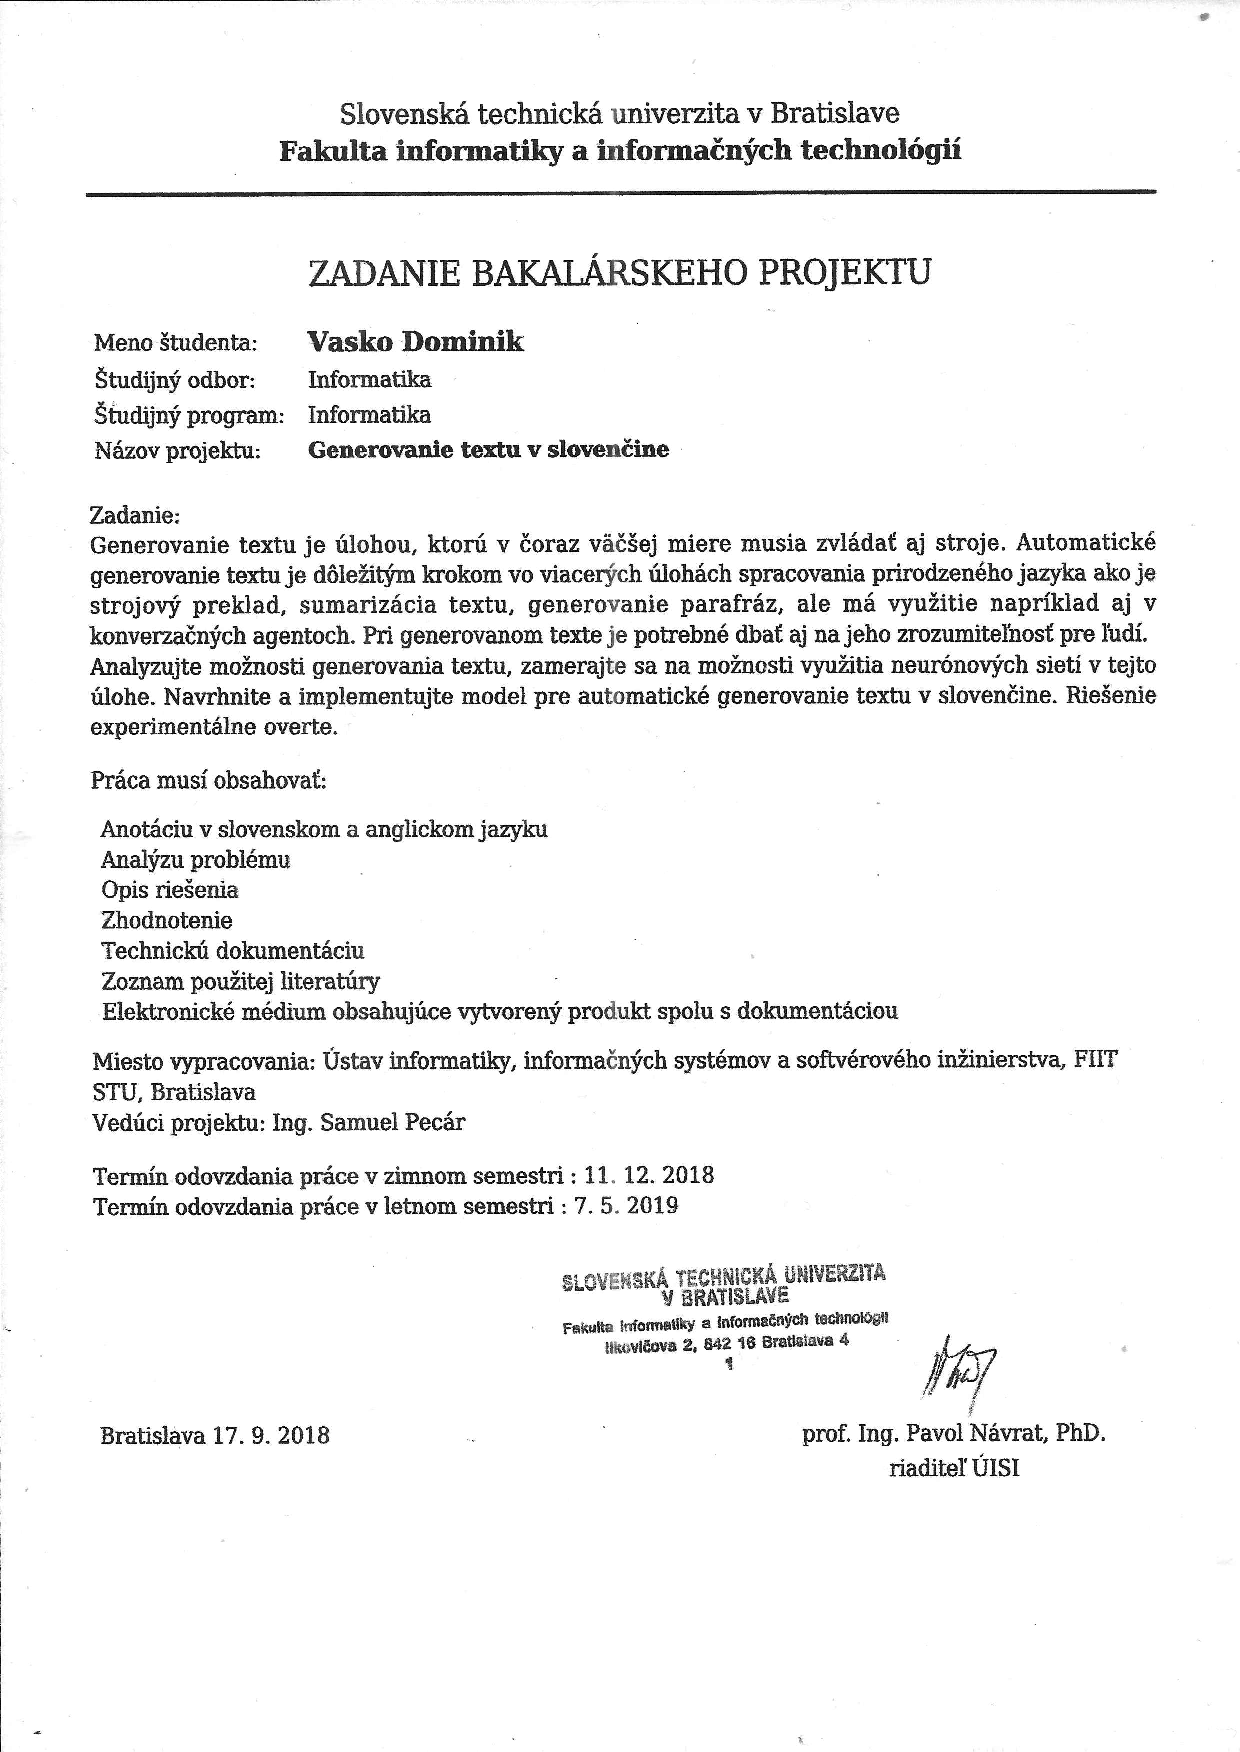
\includepdf{bct.pdf}
\afterpage{\blankpage}
\clearpage


\setcounter{page}{1}

%%
%% Declaration
%%
%% \newpage

\thispagestyle{plain}
\vspace*{15cm}
\begin{large}
\noindent
\textbf{ČESTNÉ PREHLÁSENIE} \\
\end{large}
\noindent
Čestne prehlasujem, že záverečnú prácu som vypracoval samostatne s použitím uvedenej literatúry a na základe svojich vedomostí a znalostí.
\\
\vspace*{0.5cm}\\
V Bratislave, 11.5.2017\hspace*{6.5cm}...................................\\
\hspace*{10.7cm} \Author
\cleardoublepage
\thispagestyle{plain}
\vspace*{15cm}
\begin{large}
\noindent
\textbf{POĎAKOVANIE} \\
\end{large}
\noindent
Ďakujem Ing. Samuelovi Pecárovi za odborné rady a usmernenie pri vypracovávaní mojej bakalárskej práce.
\cleardoublepage


%%
%% Anotation
%%
\newpage
\thispagestyle{plain}
\begin{center}
\begin{Large}
\textbf{Anotácia} \\
\end{Large}
\end{center}
Slovenská technická univerzita v Bratislave \\
FAKULTA INFORMATIKY A INFORMAČNÝCH TECHNOLÓGIÍ \\
\noindent
Študijný program: \Program \\
\noindent
Autor: \Author \\
\ifthenelse {\boolean{bachelor}}
{
	{Bakalárska práca: }\Title \\
}
{
	{Diplomová práca: }\Title \\
}
Vedúci práce: \Supervisor \\
\Month{ }\Year \\
\noindent
\\

V tejto práci sa budeme zaoberať generovaním textov pre ľudí, ktoré sú určený na čítanie a majú podobu prirodzeného jazyka. Práca obsahuje analýzu oblasti generovania textov prirodzeného jazyka a jednotlivých využití generovaných textov ako sumarizácia, simplifikácia, parafrázovanie a generovanie dialógov, ich vývoj a súčasný stav pre tieto úlohy.

Súčasťou práce je aj návrh a implementácia modelu na generovanie textu na ktoré budú použité hlboké rekurentné neurónové siete, ktoré dosahujú v poslednej dobe úspech v tejto oblasti a zďaleka najlepšie výsledky. Samotné generovanie textu bude robené v jazyku slovenskom a anglickom, účelom implementácie modelu v dvoch jazykoch je hlavne porovnanie rôznych prístupov pre rôzne jazyky.

Všetky experimenty budú robené na paralelných korpusoch podobnej veľkosti a z podobných voľne prístupných zdrojov ako napr. Wikipédia. Evaluácia výsledkov experimentov bude robená manuálne ľudskou silou metódou hodnotenia metrík generovaného text. Dôvodom pre manuálne hodnotenie je, že ľuďmi čitateľný text je komplexný a automatizované hodnotenie nie je vždy vhodné.

\newpage
\blankpage

\thispagestyle{plain}
\begin{center}
\begin{Large}
\textbf{Annotation} \\
\end{Large}
\end{center}
Slovak University of Technology Bratislava \\
FACULTY OF INFORMATICS AND INFORMATION TECHNOLOGIES \\
\noindent
Degree Course: Information systems \\
\noindent
Author: \Author \\
\ifthenelse {\boolean{bachelor}}
{
	{Bachelor thesis: }\mbox{Generating Slovak Texts}\\
}
{
	{Master's thesis: }\mbox{} \\
}
Supervisor: \Supervisor \\
\Year, May \\
\noindent
\\

The goal of this works is to generate text in a natural language which is readable to humans, it contains an analysis of the natural language generation field and its uses like text summarization, simplification, paraphrasing and dialog generation and their evolution.

Part of this work is a design and implementation of a model for text generation. Deep recurent neural networks will be used for that task, the reason for that is their efficiency and the fact the most state-of-the art models use them. Texts will be generated in Slovak and English languages to demostrate differences between those languages from the context of NLG.

All models used will be trained on a paralel corpuses of similar size for example from Wikipedia. The evaulation of the results will be done manualy with human power by evaluating metrics. The reason for that is mainly the complexity of natural languags where automated evaluation is not suficient.

\newpage
\blankpage

%%
%% Contents
%%
%\pagestyle{empty}

\newpage
\pagenumbering{roman}\setcounter{page}{11}

\tableofcontents{}

%%
%% Lists
%%

 \newpage
% List of Figures
 \listoffigures

% \newpage
% List of Tables
\listoftables


% \newpage
% List of Listings
%\lstlistoflistings

%%
%% Clear Page And Set New Page Counter
%%
%%\afterpage{\blankpage}
\clearpage


\pagenumbering{arabic}
\setcounter{page}{1}

\ifthenelse {\boolean{bachelor}}
{
	\sectionfont{\sectionrule{0pt}{0pt}{-2ex}{0.5pt}}
}
{
	\sectionfont{\sectionrule{0pt}{0pt}{-2ex}{0pt}}
}

%%
%% Introduction
%%
\section{Úvod}
% Text je súčasťou života každého človeka, je to jednou z dôležitých prostriedkov komunikácie myšlienok a informácií. 

% Mnoho ľudských činností v sebe zahŕňa buď vstrebávanie text zvyčajne čítaním alebo tvorbu text. Tieto činnosti môžu byť veľmi pracné a nie vždy dostatočné na obetovanie množstva času a peňazí, ktoré by bolo potrebné na ich realizáciu.

% V dnešnej dobe informačnej preťaženosti, prístupu k internetu a veľkému množstvu textu je dôležité mať spôsob ako sa s veľkým množstvom text vysporiadať a oddeliť užitočné od zbytočného.

% Aj ľudia aj stroje by profitovali z automatizácie týchto činností. Zautomatizovanie takýchto činnosti sa zaoberá NLG alebo generovanie prirodzeného jazyka.

% Môžeme nájsť viacero definícií NLG jednou z klasických je, že NLG je jednou z oborov umelej inteligencie a NLP, ktorej úlohou je zvyčajne z nejazyčných vstupov vygenerovať text pre rôzne domény a oblasti ľudských činnosti \cite{reiter_dale_2000_buildingnlgsystems}.

% V poslednej dobre sa však na rôzne úlohy hlavne text-to-text používajú prístupy, ktorých vstupom nie sú len dáta ale aj text\cite{Nallapati_2016_sum_s2s, Nisioi_2017_simpl_expl, Mallinson_2017_para_w_mt}. Rozdiel medzi touto prvotnou definíciou NLG a reálnymi aplikáciami v súčasnosti značí, že NLG prešlo počas posledných dvoch desaťročí mnohými zmenami.
% % \cite{ref1, ref2...} 

% Vo všeobecnosti ide o generovanie textu, ktorý je priamo určený na čítanie pre ľudí. Táto definícia je všeobecná a preto má NLG široké využitie. Niektoré príklady využitia NLG zahŕňajú napr. generovanie článkov do novín ako napríklad futbalové reportáže\cite{vanderlee_krahmer_wubben_2017_PASS}, zdravotnícke správy, ale aj všeobecnejšie, nezávislé od domény využitia ako simplifikácia alebo sumarizácia textu, generovanie parafráz, prekladanie textov\cite{gatt_2018_survey}.



Zrak,hmat a sluch sú tromi našimi najdôležitejšími vnemami, pomocou ktorých prijímame veľké množstvo informácií a bez ktorých by sme sa ťažko v živote zaobišli. Práve preto text, či už vo viditeľnej, hmatateľnej alebo zvukovej podobe predstavuje dôležité médium na prenášanie, komunikáciu a organizovanie dát a informácií, ktoré má hlavne v dnešnej dobe internetu a sociálnych sietí veľmi dôležitú rolu.

Čím viac sa spoločnosť blíži k viac digitálnej kde informácií je veľmi veľa bude treba tvoriť ale aj vstrebávať a organizovať viac a viac textov. Google, Wikipédia, protokoly ako html ktoré nám umožňujú prispievať obsah na internet, blogy, magazíny, knihy, noviny, väčšina obsahu na sociálnych sietiach a na internete atď. sú tvorené veľkým množstvom textov.

Nie len digitálne ale aj mnoho klasických ľudských aktivít v sebe zahŕňa tvorbu alebo vstrebávanie nejakých druhov textov či je to obyčajná medziľudská komunikácia alebo písanie na papier.

Práca s textom sa týka mnohých oborov od študentov, sekretárok až po softvérových architektov a manažérov. Aby veľké množstvo informácií nespôsobilo informačné preťaženie je treba prácu s textom automatizovať a vysporiadať sa s filtrovaním užitočných informácií od tých zbytočných, čo vedie k uľahčeniu práce mnohých ľudí.

Väčšina týchto textov je v podobe prirodzeného jazyka(slovenčina, angličtina) a majú osobnú povahu, čo môže predstavovať prekážku pri automatizácii. Lúdia veľmi jednoducho vedia rozlíšiť zlý text od dobrého.

Manuálne písanie textov môže byť náročné na realizáciu, jednak kvôli potrebe vedomostí v danej oblasti druhak, že to môže byť nudné a cenovo nevýhodné a v nektorých prípadoch, kedy je textu veľmi veľa, aj nemožné. Aj ľudia aj stroje by profitovali z automatizácie týchto činností. Zautomatizovanie takýchto činnosti sa zaoberá NLG alebo generovanie prirodzeného jazyka.

V tejto práci sa zameriame na generovanie textov konkrétne v jazyku slovenskom a anglickom. Kvôli tomu, že väčšina automatizovaní tvorenia textov je robená v angličtine. Predstavuje to niekoľko prekážok. Slovenkých textov je pomerne málo a ešte ťažšie sa získavajú, ak chceme použiť nejaký novší prístup potrebujeme veľa
vzorov na to ako text správne písať(nechceme to robiť manuálne). Navyše slovenčina je morfologicky bohatší jazyk, používa veľa prípon, predpôn a má viac časov ako angličtina. Taktiež exituje málo systémov, ktoré sa o generovanie slovenského textu pokúsili, preto budeme používať niečo, čo funguje na angličtinu ale vieme to použiť aj na slovenčinu. Z tohto vypláva aj ďalší cieľ práce a to porovnanie nejakých aktuálnych prístupov na generovanie textu v slovenčine a angličtine.

Porovnanie chceme robiť kvôli tomu, že systémy majú svoj limit a tým pádom že slovenčina je pomerne expresívny a syntakticky bohatý jazyk ako angličtina. Preto prístupy vhodne pre angličtinu alebo iný jazyk nemusia nutne byt dobré pre slovenčinu, respektíve chceme sa dozvedieť ci je nejaký signifikantný rozdiel medzi rovnakým systémom, ktorý sa učí iný jazyk.

Prínosom práce ma byť porovnanie toho či prístupy použite v iných jazykoch fungujú aj na slovenčine a či sa dá niečo zmysluplné vygenerovať. Na ohodnotenie budeme potrebovať ľudí, ktorý text ohodnotia a povedia či je dobrý na základe rôznych metrík. Dôvod pre použitie ludi je ten, že text je komplexný a automatické overenie správnosti je subjektívne, komplikované a nástroje, ktoré sú prístupné sú nepresné môžu považovať aj zlé texty za správne. 

Môžeme nájsť viacero definícií NLG jednou z klasických je, že NLG je
jednou z oborov umelej inteligencie a NLP, ktorej úlohou je zvyčajne z
nejazyčných vstupov vygenerovať text pre rôzne domény a oblasti
ľudských činnosti \cite{reiter_dale_2000_buildingnlgsystems}.

V poslednej dobre sa však na rôzne úlohy hlavne text-to-text používajú
prístupy, ktorých vstupom nie sú len dáta ale aj
text\cite{Nallapati_2016_sum_s2s, Nisioi_2017_simpl_expl,
Mallinson_2017_para_w_mt}. Rozdiel medzi touto prvotnou definíciou NLG
a reálnymi aplikáciami v súčasnosti značí, že NLG prešlo počas
posledných dvoch desaťročí mnohými zmenami.

Vo všeobecnosti ide o generovanie textu, ktorý je priamo určený na
čítanie pre ľudí. Táto definícia je všeobecná a preto má NLG široké
využitie. Niektoré príklady využitia NLG zahŕňajú napr. generovanie
článkov do novín ako napríklad futbalové
reportáže\cite{vanderlee_krahmer_wubben_2017_PASS}, zdravotnícke
správy, ale aj všeobecnejšie, nezávislé od domény využitia ako
simplifikácia alebo sumarizácia textu, generovanie parafráz,
prekladanie textov\cite{gatt_2018_survey}.

\afterpage{\blankpage}
\clearpage

%%
%% analysis
%%
\section{Generovanie Textu}

Kým výstupom NLG je skoro vždy text. Vstupom môže byť spektrum údajov. Vstupom však musí byť niečo čo chceme koncovému čitateľovi výstupným textom sprostredkovať, informovať ho. Príkladmi vstupu môžu byť číselné údaje(data-to-text) alebo text samotný(text-to-text)\cite{roger_paul_2002_whatisnlg}.

\subsection{Podúlohy pri generovaní prirodzeného jazyka}
Dosiahnutie transformácie vstupu na výstup môže byť vykonávaný rôznymi spôsobmi. Jeden z takých všeobecných prístupov opisujú Reiter a Dale vo svojej knihe\cite{reiter_dale_2000_buildingnlgsystems}. V tomto prípade je celý proces rozdelený na menšie podúlohy. Kde každá z týchto úloh vykoná istú časť transformácie vstupu. Tieto úlohy sú nasledovné Content determination, Text structuring, Sentence aggregation, reffering expression generation, lexicalization a surface realization \cite{reiter_dale_2000_buildingnlgsystems}. Toto rozdelenie sa stalo de-facto rozdelením v NLG, ktoré je dodnes používané v niektorých systémoch, Reiter k tomuto rozdeleniu dospel na základe pozorovaní a trendov v NLG systémoch.

\subsubsection{Content determination}
Alebo určovanie obsahu, slúži na určenie obsahu toho čo na konci generácie chceme čitateľovi sprostredkovať. Vstup, dataset z ktorého text generujeme môže obsahovať aj nadbytok informácií, ktoré sú irelevantné, pre naše špecifické použitie. Táto úloha je veľmi dôležitá lebo ovplyvňuje ostatné úlohy ktorú ju nasledujú, ak vyberieme málo informácií konečný text môže byť neúplný. Ďalšou s problémov je že určovanie obsahu je zvyčajne závislé od domény v závislosti čo generujem, chcem vybrať správne údaje.

Napr. pri generovaní článkov pre fanúšikov futbalu\cite{vanderlee_krahmer_wubben_2017_PASS}, sa na vstup vyberú len informácie, ktoré sa väčšinou vyskytujú v článkoch písaných ľuďmi.

 Od starších prístupov prešlo na viac automatizované prístupy pomocou strojového učenia alebo rozpoznávania vzorov. Kde sa relevantný obsah vyberá na základe korelácie výskytu slov a variácie dát\cite{perera_2017_recentnlgadv}.

\subsubsection{Text structuring}
Štrukturovanie textu slúži na zoradenie informácií získaných výberom v predchádzajúcom kroku, do správneho poradia aby dávali zmysel. Nesprávne poradie môže viesť k nezmyselnému textu, ktorý, čitateľ nebude vedieť sledovať. V Prípade futbalových článkov môžeme dáta znova organizovať do takého poradia v akom by sme to našli napr. v novinách\cite{vanderlee_krahmer_wubben_2017_PASS}. t.j. Nadpis, úvod, chronologický priebeh hry a beseda. Ak by sme začali rekapituláciu zápasu od zadu, dostali by sme článok ktorý je nezmyselný.

\subsubsection{Sentence aggregation}
Pri tejto úlohe sa stretávame s viacerými definíciami. ako odstránenie redundantných informácií alebo určenie blízkosti jednotlivých údajov(v jednej vete alebo vo viacerých)\cite{gatt_2018_survey}. Výsledok je však rovnaký urobiť text kompaktnejším aby bol ľahšie a lepšie čitateľní. Môže to znamenať rozdiel medzi piatimi vetami kde sa mení iba predmet vety a jednou vetou kde všetky tieto predmety sú vyjadrené jedným slovom alebo spojené spojkami\cite{Dalianis_1996_lexagr_ord}. V praxi to môže znamenať rozdiel medzi nasledujúcimi výstupmi.

\begin{itemize}
    \item Tomáš mal v pondelok na raňajky jablko.
    \item Tomáš mal v nedeľu na raňajky jablko.
\end{itemize}

\begin{itemize}
    \item Tomáš mal celý týždeň na raňajky jablká.
\end{itemize}

\subsubsection{Lexicalization}
Leksikalizácia znamená nájdenie správnych slov na vyjadrenie informácií v texte. Jazyky zvyčajne majú synonyma, pomocou ktorých môžeme text plynulejšie vyjadriť. Opakovanie rovnakých výrazov môže pôsobiť repetitívne a nudne\cite{gatt_2018_survey}.

\subsubsection{Referring expression generation}
Generovanie odkazujúcich výrazov(Reffering Expression Generation), slúži na tvorbu správnych odkazov pre jednotlivé veci v texte, hlavne kvôli rozlíšiteľnosti. Je to zvyčajne diskriminačná činnosti pri ktorej jednotlivé doménové entity špecifikujeme dovtedy, kým ich vieme od ostatných entít rozoznať\cite{reiter_dale_2000_buildingnlgsystems}.

\subsubsection{Surface realization}
Poslednou úlohou je samotné generovanie gramatický, syntaktický a morfologický správneho a konkrétneho textu. Slúži na pretavenie abstraktných reprezentácií ktoré sme doteraz zo vstupu získali do konkrétneho jazyka\cite{gatt_2018_survey}.

Najjednoduchšie sa dá spraviť šablónami alebo predurčenými statickými spravami(canned text) tieto prístupy sú však primitívne a nedostatočné. Prístupy, ktoré sa používajú sú zvyčajne založené na štatistických princípoch alebo na základe rôznych gramatík(CCG, SGS)\cite{perera_2017_recentnlgadv}.

\subsection{Krátka história NLG}
Prvé systémy, ktoré sa objavujú v 60. rokoch slúžili hlavne na preklad textov z rôznych jazykov. Vo väčšine prípadov vykonávali iba surface realization. Až neskôr v 70. rokoch sa objavujú systémy na generovanie textu z ne-lingvistických údajov. Tieto systémy poukazovali na to že NLG nie je len NLU odzadu a taktiež na vznik istých problémov pri NLG. 80. roky predstavujú obdobie rozvoja NLG, odstupovalo sa od stavania monolitických systémov a pristúpilo sa k skúmaniu jednotlivých podúloh pri generovaní\cite{reiter_dale_2000_buildingnlgsystems}. Koncom 90. rokov väčšina architektúr používala pipeline(rúrovú) architektúru s menšími zmenami. Tieto architektúry boli podobné aj naprie tomu, že mali rozdielne teoretické pozadia(východiská?). Taktiež rozdeľovali generovanie na podobné podúlohy. Táto podobnosť pravdepodobne súvisí s tým ako ľudský mozog vytvára hovorenú reč aj keď podobnosť k psycholingvistike nebol cieľom týchto systémov.

Rúrová architektúra sa teda stala de facto štandardom\cite{reiter_1994_consensusarch}. Je mnoho dôvodov prečo rúrovú architektúru používať. Jedným z nich je jej jednoduchosť a jednoduchosť implementácie a následné odhaľovanie chýb. Vývoj takýchto systémov stojí menej námahy ako vytvárať komplexné systémy. Aj keď majú svoje nedostatky ako napríklad absencia spätnej väzby.

\subsection{Úlohy v NLG}
Okrem horeuvedených podúloh existujú aj iné prístupy, ktoré v sebe nezahŕňajú modulárne systéme. Sem patria metódy založené na strojovom učení a neuŕonových sietiach, ktoré sa učia vzťah medzi vstupnými a výstupnými údajmi. Nasleduje zopár populárnych využití NLG, sú to hlavne využitia pre úlohy typu text-to-text. Aj keď podobné prístupy môžeme použiť aj na klasické data-to-text generovanie\cite{Lapouras_2016_Imitation}.

\subsubsection{Parafrázovanie}
Parafrázovanie alebo prerozprávanie toho istého obsahu inými slovami. Je užitočná činnosť, ktorá má mnoho využití v kombináciou s ostatnými úlohami NLG ako sumarizácia, odpovedanie otázok(question answering), strojový preklad a.i \cite{Colin_2018_para}\cite{Mallinson_2017_para_w_mt}.
Prístupy k parafrázovaniu môžeme rozdeliť na monolingvistiské, pivotné metódy a neurónové prístupy. V porovnaní prístupov metóda založená na neurónovoých prístupoch mala lepšie výsledky ako klasické modely založené na frázach\cite{Mallinson_2017_para_w_mt}.

\subsubsection{Simplifikácia}
   Simplifikácia textu znamená zmenu jazykovej štruktúry pričom informácie, ktoré sú v tomto texte obsiahnuté ostávajú rovnaké, zmysel textu sa nemení. Hlavnou motiváciou pre simplifikácia je sprístupnenie informácií menej vzdelaným ľuďom, deťom, cudzincom, alebo osobám s rôznymi poruchami ,ktoré im sťažujú pochopenie text ako napr. dyslexia alebo ľudia trpiaci hluchotou \cite{Inui_2003_simpl_assist}.
   
   Slabší čitatelia môžu mať problémy s čítaním komplikovanejších textov keď sa mozog musí sústrediť na spracovávanie slov vyššie kognitívne činnosti trpia. Ľudia trpiaci takýmito poruchami musia použiť väčšiu časť pamäte na pochopenie textu. Rozdelenie viet na kratšie časti spôsobuje odbremenenie od pamätanie si, a zjednodušuje čítanie. Je dokázané, že metódy manuálnej simplifikácie textu pomáhajú slabším čitateľom. Práve tieto štúdia motivovali výskum automatizovanej simplifikácie textu\cite{siddharthan_2014_simpl}.
   
   Okrem ľudí simplifikácia textu môže predstavovať rôzne výhodu aj pre systémy, ktoré s textom extenzívne pracujú ako napríklad systémy na strojový preklad\cite{Chandrasekar_1996_simpl_moti}.
    
    Tak ako aj vo viacerých oblastiach NLG aj pri simplifikácii sa v poslednej dobe prechádza od klasických prístupov založených na gramatikách, ručne písaných pravidlách na používanie neurónové siete, konkrétne modely typu sequence-to-sequence, ktoré dosahujú lepšie výsledky ako doteraz známe systémy \cite{Nisioi_2017_simpl_expl}. Tieto systému sa učia end-to-end, a majú jednoduchšie architektúry ako klasické systémy založené na rôznych štatistických prístupoch, umožňuje to trénovanie modelov na základe znakov alebo aj vo viacerých jazykoch. Oproti prvotným systémov tieto pristupujú k celej úlohe simplifikácie ako k prekladu jazyka do jeho zjednodušenej podoby.
    
    Populárnou trénovacou sadou pre simplifikáciu textov sú jednak manuálne simplifikované texty (gigaword duc etc.) alebo paralelné korpusy napr. Anglická wikipédia a jej simplifikovaná alternatíva\cite{Coster_2011_simpl_en_wiki}.

\subsubsection{Sumarizácia}
    Sumarizácia má za úlohu skrátiť text za účelom znížiť množstvo textu na čítanie pričom sa zachovajú dôležité informácie v texte. Hlavnou motiváciou pre takéto systémy je zníženie informačného preťaženia v dobe internetu a ľahko prístupných informácií\cite{nenkova_2011_autosum}.
    
    Jedna z prvých pokusov o sumarizácia, ktorá sa zaoberala tvorbou abstraktov z vedeckých textov, fungovala na základe toho ako často sa jednotlivé slová vyskytujú a na základe tejto metriky sa vybrali vety, ktoré sa použijú v koncovom texte \cite{luhn_1958_autoabstract}. Tento prístup je založený na tom, že autor ktorý dielo píše bude dôležité slová opakovať, a nebude mať dostatok synonym. Celá sumarizácia sa potom zakladá na extrakcii viet.
    
    Okrem extrakcie poznáme aj ďalšie prístupy ako kompresia alebo abstrakcie\cite{nenkova_2011_autosum}. Avšak kvôli tomu, že väčšina ľudských sumárov je viac abstraktných, spôsoby kde sa vyberajú slová a vety z pôvodného textu sú nedostatočné. Je za potreby text pochopiť a následne abstraktnú myšlienku vyjadriť textom \cite{Banko_2004_ngrams}.
    
    V prípade abstraktívnej sumarizácie dosahujú najlepšie výsledky neurónové siete typu sequence-to-sequence \cite{Piji_2017_deep_abs_sum}\cite{Nallapati_2016_sum_s2s}.

\subsubsection{Generovanie dialógov}
Dialógové systémy majú za úlohu generovať odpovede pre zadané otázky. Využitie takýchto systémov je možné napríklad pri chatbotoch, ktoré majú za úlohu komunikovať s užívateľom v prirodzenom jazyku.

Klasické prístupy v sebe zahŕňali výber odpovede z databázy odpovedí. Tieto prístupy majú malú úroveň generalizácie a možnosti odpovedí sú limitované tým pádom, že sa odpovedá na základe pravidiel\cite{AbuAli_2016_Botta}.

Novšie prístupy zahŕňajú založené na štatistickom strojovom učení v sebe zahŕňajú učenie sa vzťahov medzi otázkami a odpoveďami na základe nejakého korpusu. Tieto prístupy sú automatizované a jediné čo potrebujeme sú páry - otázky, odpovede. Najlepšie na realizácie takýchto úloh sú znova sequence-to-sequence modely. Ktoré dosahujú vylepšené výsledky oproti starším spôsobom\cite{Wu_2018_dialog}.

\subsection{NLG pomocou deep learningu}
Ako sme mohli vidieť mnoho state of the art systémov používajú neurónové siete. Tieto prístupy sa stávajú viac a viac populárnymi hlavne v dnešnej dobe keď je prístupným mnoho dát a korpusov.

Ako však použijeme neurónové siete? Tým pádom, že naším cieľom je použiť text ako vstup a z neho generovať text. budeme potrebovať architektúru neurónových sietí, ktorá je na túto úlohu vhodná. Klasické neurónové siete s kladnou spätnou väzbou nie sú dostatočné na spracovanie sekvenčných vstupov.

Pre spracovanie sekvenčných dát (hudba, text atď.) je vhodné používať rekurentné architektúry, hlavnou výhodnou je že tieto architektúry robia rozhodnutia aj na základe vstupov ktoré už dostali, nie len na základe aktuálneho vstupu. Klasické RNN siete trpia miznúcim alebo explodujúcim gradientom\cite{pascanu_2013_difficulty}, ktorý je technický problém ktorý nastáva pri propagácia chyby a gradient jednoducho stráca, na adresovanie týchto nedostatkov boli vyvinuté architektúry ako GRU\cite{cho_2014_learning} alebo LSTM\cite{hochreiter_1997_long} s tzv. hradlami(gates) ktoré kontrolujú čo si neurón má zapamätať alebo zabudnúť. Všetky tieto neurónky majú za úlohy naučiť sa pravdepodobnostnú funkciu, ktorá zachytáva závislosť medzi vstupmi a výstupmi.

Viacero text-to-text NLG úloh majú na vstupe aj výstupe sekvenciu znakov, pre tieto vieme použiť špeciálne architektúry sequence-to-sequnce. Tieto architektúry sa zvyčajne skladajú z dvoch vrstiev jedného enkódera a dekodéra\cite{sutskever_2014_sequence}.
\clearpage
%%
%% analysis
%%
%%\input{03-taxonomy.tex}
%%\clearpage
%%
%% diploma goal
%%
\section{Cieľ Práce}
Cieľom tejto prace bude generovať text v prirodzenom jazyku, t.j. určený pre ludi na čítanie. Využitie takéhoto systému potom môže byt rôznorodé, slúži hlavne na automatizovanie prace pri písaní textov. A automatizovanie rôznych úloh na ktoré bolo treba robiť v minulosti manuálne sem spadajú už zmienené úlohy simplifikácie, sumarizácie, strojového prekladu, parafrázovania a. i.

Pozrieme sa na oblasť NLG ako sa vyvíjala a aké v nej majú využitia neuronové siete. Generovanie bude teda robene cez neuronové siete, hlavne kvôli dostupnosti veľkých množstiev dát a jednoduchosti ich použitia a trénovania. Ich výkon je tiež porovnateľný s inými metódami v NLG, navyše odstraňujú mnoho nevýhod starších prístupov.

Hodnotenie výsledkov generovania bude robené na základe metrík, ale kvôli komplexnosti prirodzeného jazyka a ťažkosti určenia objektívnej kvality textu text bude vyhodnotený aj manuálne.

Pre túto prácu sme si stanovili nasledovné ciele:

Analyzovať oblasť NLG a možnosti na generovanie textu
\begin{itemize}
    \item Zistiť čo v sebe generovanie textu zahŕňa
    \item Navrhnúť a implementovať model na generovanie
\end{itemize}

Využitím NN natrénovať modely, ktoré sú schopné generovať text.
\begin{itemize}
    \item vyhodnotenie výsledkov trénovanie na slovenskom aj anglickom texte z kvalitatívneho hľadiska
    \item Trénovanie na paralelných korpusoch
\end{itemize}

\afterpage{\blankpage}
\clearpage
%%
%% design
%%
\section{Návrh}

% prva uroven abstrakcie
Chceme pomocou neurónovej siete namodelovať funkciu ktorá nám povie, po istom počte písmen aké je najpravdepodobnejšie ďalšie písmeno. Takýmto spôsobom budeme vedieť generovať texty. Celý proces môžeme rozdeliť na dve podúlohy, prvá je trénovanie modelu, kedy sa model učí a druhá podúloha je generovanie, pri ktorom model na základe naučeného predpovedá.

Na trénovanie budeme potrebovať dáta, z ktorých sa náš model vie naučiť pravdepodobnostné rozloženie písmen. Pre tento prípad sme si zvolili Wikipédiu, kvôli svojej rozmanitosti a veľkosti. Model na vstup dostane sekvenciu znakov a bude musieť predpovedať sekvenciu znakov posunutú o jeden znak ďalej, takto sa naučí ako z aktuálnej sekvencie vygenerovať ďalšiu sekvenciu s pridaným znakom.

Na generovanie si môžeme vstupnú sekvenciu vymyslieť, môže to byť písmeno alebo celé slovo. A už trénovaná sieť bude vedieť povedať, pravdepodobnosti toho aké by malo byť ďalšie písmeno v poradí. Príkladom môže byť že mu na vstup zadáme sekvenciu "abc" a sieť vráti pravdepodobnosti pre celý slovník v tomto prípade iba a,b,c s prislúchajúcimi hodnotami ich pravdepodobnosti výskytu ako ďalšie písmeno(napr. 0.2, 0.2, 0.6) potom je už na nás, ktoré si vyberieme a ako.

% Budeme trénovať neurónovú sieť a našim cieľom bude namodelovať pravdepodobnostné rozloženie jednotlivých písmen v slovenčine a angličtine a následne pomocou tohto štatistického rozdelenia generovať n-gramy t.j. text znak po znaku pričom budeme brať do úvahy nie len predchádzajúce prímeno ale všetky predchádzajúce písmená. Návrh sa teda skladá z dvoch častí z trénovania a následného generovanie. Pri trénovaní získame pravdepodobnostné rozdelenie písmen a pri generovaní pomocou tohto rozdelenia budeme predpovedáme nasledujúce písmeno v poradí.

% druha uroven abstrakcie
% dataset
% model obr

\subsection{Dataset}
% Z IITSRC

\subsection{Opis Modelu}
Tým pádom že modelujeme sekvenciu znakov a závisí nám aj od predchádzajúcich  vstupoch nie len na konkrétnom použijeme rekurentnú neurónovú sieť. Konkrétne LSTM siete, ktoré nemajú problém s dlhodobými závislosťami vstupov.

Na modelovanie a generovanie použijeme model znázornení na obrázku \ref{fig:nn_model}. Vstup do siete bude kódovaní ako one-hot vektor (každé písmeno má priradení index) tento vstup sa posunie do Embedding vrstvy, ktorá má za úlohu naučiť sa vektorové reprezentácie pomocou desatinnými číslami pre jednotlivé vstupy, táto reprezentácia sa potom posunie do LSTM vrstvy. Nakoniec výstup posunieme do lineárnej vrstvy ktorá nám zredukuje výstup z LSTM vrstiev na vhodnú veľkosť, ktorý potom môžeme interpretovať ako vektor pravdepodobnostných hodnoty pre jednotlivé možné vstupy.

Konfigurácia siete je nasledujúca:
embedding vrstva nám vráti vektor s 200 dimenziami
máme 2 vrstvy LSTM sietí, s veľkosťou 200 neuŕonov
a na konci použijeme softmax

\subsection{Trénovanie Modelu}

Náš model budeme trénovať na slovenskom a anglickom texte, korpus použijeme z wikipédie. Kvôli rozdielom vo veľkosti slovenskej a anglickej wikipédie použijeme voľne dostupné texty slovenskej a simplifikovanej anglickej wikipédie.

Trénovanie siete potom prebieha tak že každému písmenu pridelíme index(one-hot vektor) zo slovníka a následne ich pošleme do nášho modelu. Výslednú hodnotu porovnáme s ďalšou v poradí, váhy sa vhodne upravia

Celú sieť trénujeme na slovenskej a anglickej wikipédie. Kvôli rozdielom vo veľkosti a kvality slovenskej a anglickej wikipádii použijeme len simple english wikipédiu, ktorá má porovnateľnú veľkosť.

\subsection{Generovanie Textu}
V tejto fáze natrénovanej sieti pošleme písmeno a z výstupu siete zistíme písmeno s najvyššou hodnotou pravdepodobnosti, ktoré sa by sa mohlo vyskytnúť po vstupe tento výstup použijeme ako ďalší vstup do siete, takto pokračujeme, kým nemáme dostatočné množstvo textu viď obr. \ref{fig:nn_gen}.
% \begin{table}[]
% \begin{tabular}{|l|}
% \hline
% \begin{tabular}[c]{p{\linewidth}}John Cheerny\\John Leyn Show (August 24, 1940 0 February 23, 1987) was an American singer-songwriter and worldwide. He acted in the band for songs for the 1990s to the "Michael Albert Andrew \& Ort". He was set during the mid-1990s. He won a former club which became a character for the business Adele Shelley dollar women's song book "Raw" as NXT War Railway from the 2001 census.
% \end{tabular} \\ \hline
% \begin{tabular}[c]{p{\linewidth}}Saint-Martin\\ Saint-Maritre je francúzska obec, ktorá sa nachádza v departemente Orne, v regióne Dolná Normandia.\\ Obec má rozlohu . Najvyšší bod je položený a najnižší bod\\ Počet obyvateľov obce je ().\\ Nasledujúci graf zobrazuje vývoj počtu obyvateľov v obci.\end{tabular}                                                                                                                        \\ \hline
% \end{tabular}
% \caption{\label{tab:gen-text}Ukážka vygenerovaného slovenského a anglického textu.}
% \end{table}

\usetikzlibrary{positioning}

% \begin{figure}[ht]
% \centering



% \begin{tikzpicture}
% 	\node[rectangle] (Y0) at (0, 0) {$\dots$};
	
% 	\node[rectangle, draw, right=2em of Y0, minimum height=1cm, minimum width=1cm] (RNN) {NN};
% 	\node[rectangle, right=of RNN, draw, minimum height=1cm, minimum width=1cm] (RNN2) {NN};
% 	\node[rectangle, right=of RNN2, draw, minimum height=1cm, minimum width=1cm] (RNN3) {NN};
% 	\node[rectangle, right=2em of RNN3] (RNN4) {$\dots$};
			
% 	\node[below=of RNN] (X1) {'c'};
% 	\node[below=of RNN2] (X2) {'a'};
% 	\node[below=of RNN3] (X3) {'t'};
	
% 	\node[above=of RNN] (Y2) {'a'};
% 	\node[above=of RNN2] (Y3) {'t'};
% 	\node[above=of RNN3] (Y4) {'.'};
			
% 	\draw[-stealth, thick] (X1) -- (RNN);
% 	\draw[-stealth, thick] (RNN) -- (Y2);
	
% 	\draw[-stealth, thick]
% (RNN) edge[out=90,in=270, looseness=2] node[pos=0.55,yshift=5pt] {} (RNN2);

%     \draw[-stealth, thick] (X2) -- (RNN2);
% 	\draw[-stealth, thick] (RNN2) -- (Y3);

% 	\draw[-stealth, thick]
% (RNN2) edge[out=90,in=270, looseness=2] node[pos=0.55,yshift=5pt] {} (RNN3);

%     \draw[-stealth, thick] (X3) -- (RNN3);
% 	\draw[-stealth, thick] (RNN3) -- (Y4);

% 	\node[below=4em of Y0] (d) {\dots};
% 	\node[below=4em of RNN4] (d) {\dots};
% \end{tikzpicture}
%     \caption{Spôsob generovanie písmen na základe predchádzajúcich písmen}
%     \label{fig:nn_gen}
% \end{figure}

\begin{figure}[H]
\begin{center}
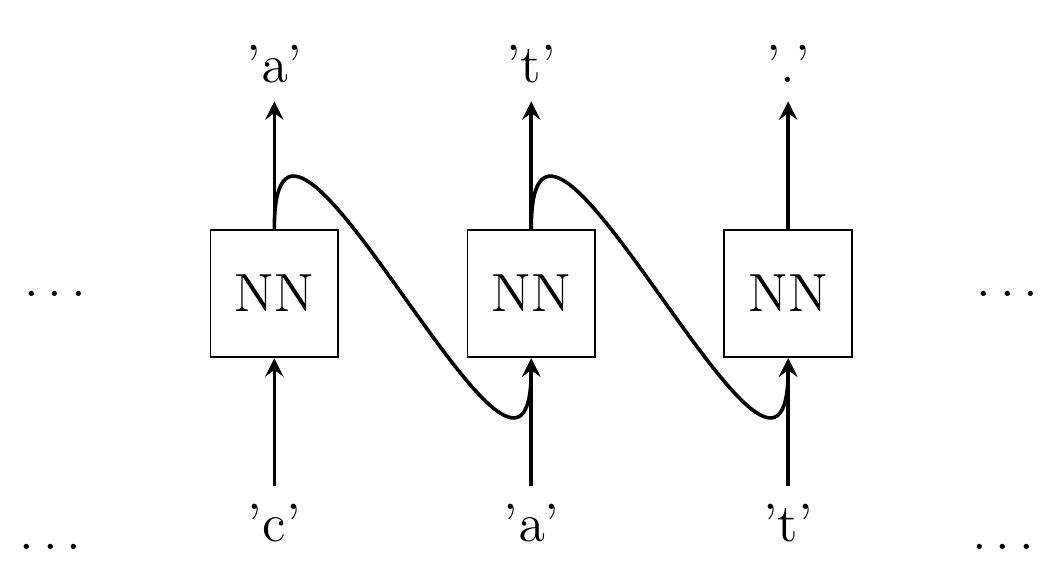
\includegraphics[width=1.0\linewidth]{figures/model-2.png}
\caption{Spôsob generovanie písmen na základe predchádzajúcich písmen}
\label{fig:nn_gen}
\end{center}
\end{figure}

% \begin{figure}[ht]
% \centering


% \begin{tikzpicture}
% 	\node[rectangle] (Y0) at (0, 0) {$\dots$};
	
% 	\node[rectangle, draw, right=2em of Y0, minimum height=1cm, minimum width=1cm] (RNN) {LSTM};
% 	\node[rectangle, right=of RNN, draw, minimum height=1cm, minimum width=1cm] (RNN2) {LSTM};
% 	\node[rectangle, right=of RNN2, draw, minimum height=1cm, minimum width=1cm] (RNN3) {LSTM};
% 	\node[rectangle, right=2em of RNN3] (RNN4) {$\dots$};
			
% 	\node[rectangle, above=of RNN, draw, minimum height=1cm, minimum width=1cm] (R22) {LSTM};
% 	\node[rectangle, right=of R22, minimum height=1cm, minimum width=1cm, draw] (R23) {LSTM};
% 	\node[rectangle, right=of R23, draw, minimum height=1cm, minimum width=1cm] (R24) {LSTM};
	
% 	\node[rectangle, above=of R22, draw, minimum height=1cm, minimum width=1cm] (LIN1) {Linear};
% 	\node[rectangle, above=of R23, draw, minimum height=1cm, minimum width=1cm] (LIN2) {Linear};
% 	\node[rectangle, above=of R24, draw, minimum height=1cm, minimum width=1cm] (LIN3) {Linear};
	
% 	\node[rectangle, below=of RNN, draw, minimum height=1cm, minimum width=1cm] (EMB1) {Embed};
% 	\node[rectangle, below=of RNN2, draw, minimum height=1cm, minimum width=1cm] (EMB2) {Embed};
% 	\node[rectangle, below=of RNN3, draw, minimum height=1cm, minimum width=1cm] (EMB3) {Embed};

% 	\node[rectangle, left=2em of R22] (R21) {$\dots$};
% 	\node[right=2em of R24] (Y20) {$\dots$};
			
% 	\node[below=of EMB1] (X1) {$\vec{x}_{t-1}$};
% 	\node[below=of EMB2] (X2) {$\vec{x}_t$};
% 	\node[below=of EMB3] (X3) {$\vec{x}_{t+1}$};
% 	\node[above=of LIN3] (Y4) {$\vec{y}_{t+1}$};
% 	\node[above=of LIN2] (Y3) {$\vec{y}_t$};
% 	\node[above=of LIN1] (Y2) {$\vec{y}_{t-1}$};
			
% 	\draw[-stealth, thick] (X1) -- (EMB1);
% 	\draw[-stealth, thick] (X2) -- (EMB2);
% 	\draw[-stealth, thick] (X3) -- (EMB3);
% 	\draw[-stealth, thick, densely dotted] (Y0) -- (RNN);
	
% 	\draw[stealth-, thick] (RNN2) -- node[above, pos=0.55] {$\vec{h^1}_{t-1}$} (RNN);
% 	\draw[stealth-, thick] (RNN3) -- node[above, pos=0.55] {$\vec{h^1}_t$} (RNN2);
	
% 	\draw[-stealth, densely dotted, thick] (RNN3) -- (RNN4);
% 	\node[below=4em of Y0] (d) {\dots};
% 	\node[below=4em of RNN4] (d) {\dots};

% 	\draw[-stealth, thick] (LIN1) -- (Y2);
% 	\draw[-stealth, thick] (LIN2) -- (Y3);
% 	\draw[-stealth, thick] (LIN3) -- (Y4);
	
% 	\draw[-stealth, thick] (R22) -- (LIN1);
% 	\draw[-stealth, thick] (R23) -- (LIN2);
% 	\draw[-stealth, thick] (R24) -- (LIN3);
	
% 	\draw[-stealth, thick] (EMB1) -- (RNN);
% 	\draw[-stealth, thick] (EMB2) -- (RNN2);
% 	\draw[-stealth, thick] (EMB3) -- (RNN3);
		
% 	\draw[stealth-, densely dotted, thick] (R22) -- (R21);
% 	\draw[stealth-, thick] (R23) -- node[above, pos=0.55] {$\vec{h^2}_{t-1}$} (R22);
% 	\draw[stealth-, thick] (R24) -- node[above, pos=0.55] {$\vec{h^2}_t$} (R23);
% 	\draw[-stealth, densely dotted, thick] (R24) -- (Y20);	
			
% 	\draw[stealth-, thick] (R22) -- node[left, pos=0.55] {$\vec{o^1}_{t-1}$}(RNN);
% 	\draw[stealth-, thick] (R23) -- node[left, pos=0.55] {$\vec{o^1}_t$}(RNN2);
% 	\draw[stealth-, thick] (R24) -- node[left, pos=0.55] {$\vec{o^1}_{t+1}$}(RNN3);
	
% 	\draw[stealth-, thick] (LIN1) -- node[left, pos=0.55] {$\vec{o^2}_{t-1}$}(R22);
% 	\draw[stealth-, thick] (LIN2) -- node[left, pos=0.55] {$\vec{o^2}_t$}(R23);
% 	\draw[stealth-, thick] (LIN3) -- node[left, pos=0.55] {$\vec{o^2}_{t+1}$}(R24);
% \end{tikzpicture}

%     \caption{Model neurónovej siete na generovanie textu}
%     \label{fig:nn_model}
% \end{figure}

\begin{figure}[H]
\begin{center}
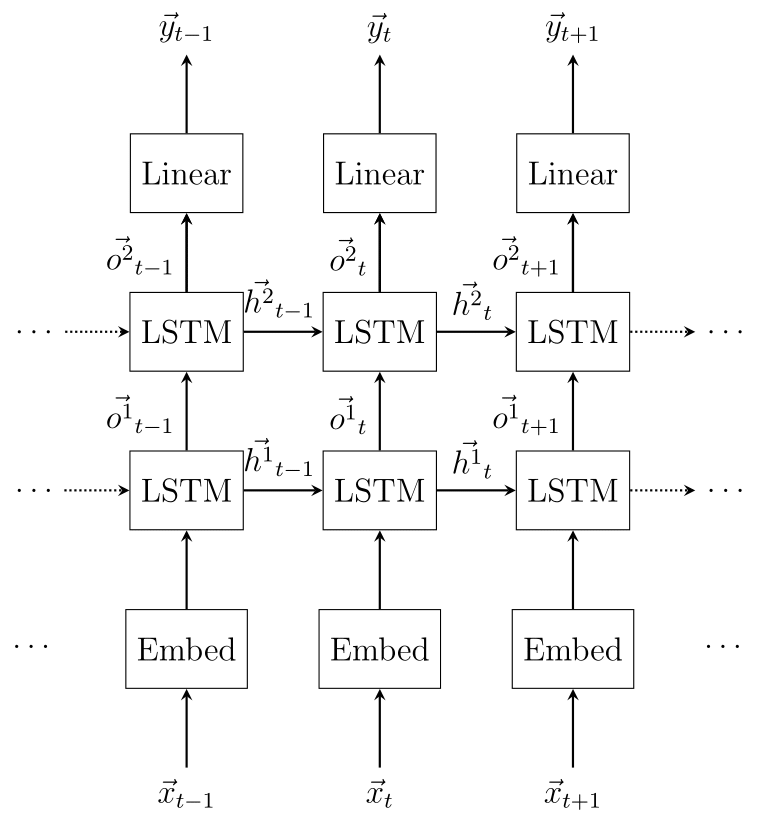
\includegraphics[width=1.0\linewidth]{figures/model-1.png}
\caption{Model neurónovej siete na generovanie textu}
\label{fig:nn_model}
\end{center}
\end{figure}

% tretia uroven abstrakcie - kod

\subsection{implementácia}
Na implementáciu použijeme programovací jazyk Python a na uľahčenie práce s neurónovými sieťami knižnicu PyTorch, ktorá obsahuje väčšinu potrebných komponentov na poskladanie modelu.

\subsubsection{predspracovanie}
% IITSRC

\subsubsection{model}
% model.py

\subsubsection{trénovanie}
% train.py

\subsubsection{generovanie}
% generate.py
\afterpage{\blankpage}
\clearpage
%%
%% test
%%
\section{Vyhodnotenie}
Výsledky experimentu budú vyhodnotené manuálne. Na vyhodnotenie sme každému testerovi dali 6 vygenerovaných textov, pričom sa vyhodnocovali tieto 4 kvalitatívne parameter textu:

\begin{itemize}
    \item Správnosť jednotlivých slov
    \item Morfologický tvar slov
    \item Slovosled
    \item Zmysluplnosť celého textu
\end{itemize}

Tieto metriky sú v poradí od najkratšej závislosti písmen až po najdlhšie. Spôsob vyhodnotenia bude nasledovný, zoberieme všetky odpovede zvlášť pre slovenský a anglický text a vytvoríme z nich priemer.

\subsection{Anglický text}
Výsledky hodnotenie anglických textov sú nasledovné:
Zhruba 79\% vygenerovaných slov dávalo zmysel
Slovosled bol správny v 40\% textov
Morfológia v prípade 66\%
A zmysel dávalo len 23\% z celkových textov

V prípade angličtiny mala naša sieť problém hlavne zachovať nejakú zmysluplnú myšlienku, kým slová a ich tvary boli pomerne dobré, sieť nedokázala zachovať dostatočný súvis pre vety a celkové články.

\subsection{Slovenský text}
Výsledky hodnotenie slovenských textov sú nasledovné:
Zhruba 69\% vygenerovaných slov dávalo zmysel
Slovosled bol správny v 58\% textov
Morfológia v prípade 54\%
A zmysel dávalo len 17\% z celkových textov

Skoro v každej metrike bola slovenčina horšia, pravdepodobne kvôli rozdielu medzi komplexnosťami jazykov. Slovenčina má pestrejšiu morfológiu a slová sa dajú ohýbať do viacerých tvarov.

Z výsledkov hodnotenia vyplýva, že aj napriek jednoduchosti nášho modelu bol schopný sa naučiž krátkodobé závisloti ktoré nám dávali zmysluplné slová, čo sa týka komplikovanejších vecí ako súvis a závislosť jednotlivých častí textov, na ktoré sa siet potrebuje naučiť dlhšie závisloti, sieť nebola schopná zapamätať si vzťahy, pomohla by asi pozornosť.


\begin{table}[]
\begin{tabular}{|l|}
\hline
\begin{tabular}[c]{p{\linewidth}}John Cheerny\\John Leyn Show (August 24, 1940 0 February 23, 1987) was an American singer-songwriter and worldwide. He acted in the band for songs for the 1990s to the "Michael Albert Andrew \& Ort". He was set during the mid-1990s. He won a former club which became a character for the business Adele Shelley dollar women's song book "Raw" as NXT War Railway from the 2001 census.
\end{tabular} \\ \hline
\begin{tabular}[c]{p{\linewidth}}Saint-Martin\\ Saint-Maritre je francúzska obec, ktorá sa nachádza v departemente Orne, v regióne Dolná Normandia.\\ Obec má rozlohu . Najvyšší bod je položený a najnižší bod\\ Počet obyvateľov obce je ().\\ Nasledujúci graf zobrazuje vývoj počtu obyvateľov v obci.\end{tabular}                                                                                                                        \\ \hline
\end{tabular}
\caption{\label{tab:gen-text}Ukážka vygenerovaného slovenského a anglického textu.}
\end{table}
\clearpage
%%
%% Conclusion
%%
%%\input{07-conclusions.tex}

%%
%% References
%%
\newpage
\addcontentsline{toc}{section}{\refname}
\bibliographystyle{acm}
\begin{flushleft}
\bibliography{references}
\end{flushleft}
\afterpage{\blankpage}
\clearpage

%%
%% Appendix
%%
\appendix
\renewcommand{\thesubsection}{\Alph{subsection}}
%%\input{08-appendix.tex}
\end{document}

%%%%%%%%%%%%%%%%%%%%%%%%%%%%%%%%%%%%%%%%%%%%%%%%%%%%%%%%%%%%%%%%%%%%%%%%%%%%%%%%%%%%%%%%

